% !TEX root = ../MasterThesis.tex

\chapter{グラフニューラルネットワークによるクラスタリング解析} \label{sec:BeamTest}

本章では、カロリメータクラスタリングに対して適用したネットワークおよび損失関数に関する技術の概要を説明し、ILCの検出器シミュレーションに対して適用した際のクラスタリング性能について示す。
4.1節では、今回使用した深層学習アーキテクチャについてその全体像を説明する。4.2節では今回使用したネットワークであるGravNetについて述べる。4.3節では、クラスタリング性能を高めるために使用した Object Condensation技術について解説する。最後に、4.4節では近接する2光子イベントをILC検出器シミュレーションで作成し、そのクラスタリング性能を評価した。

\section{深層学習アーキテクチャ}
今回用いた深層学習アーキテクチャを図\ref{GravArc}に示す。
\begin{figure}[H]
	\begin{center}
		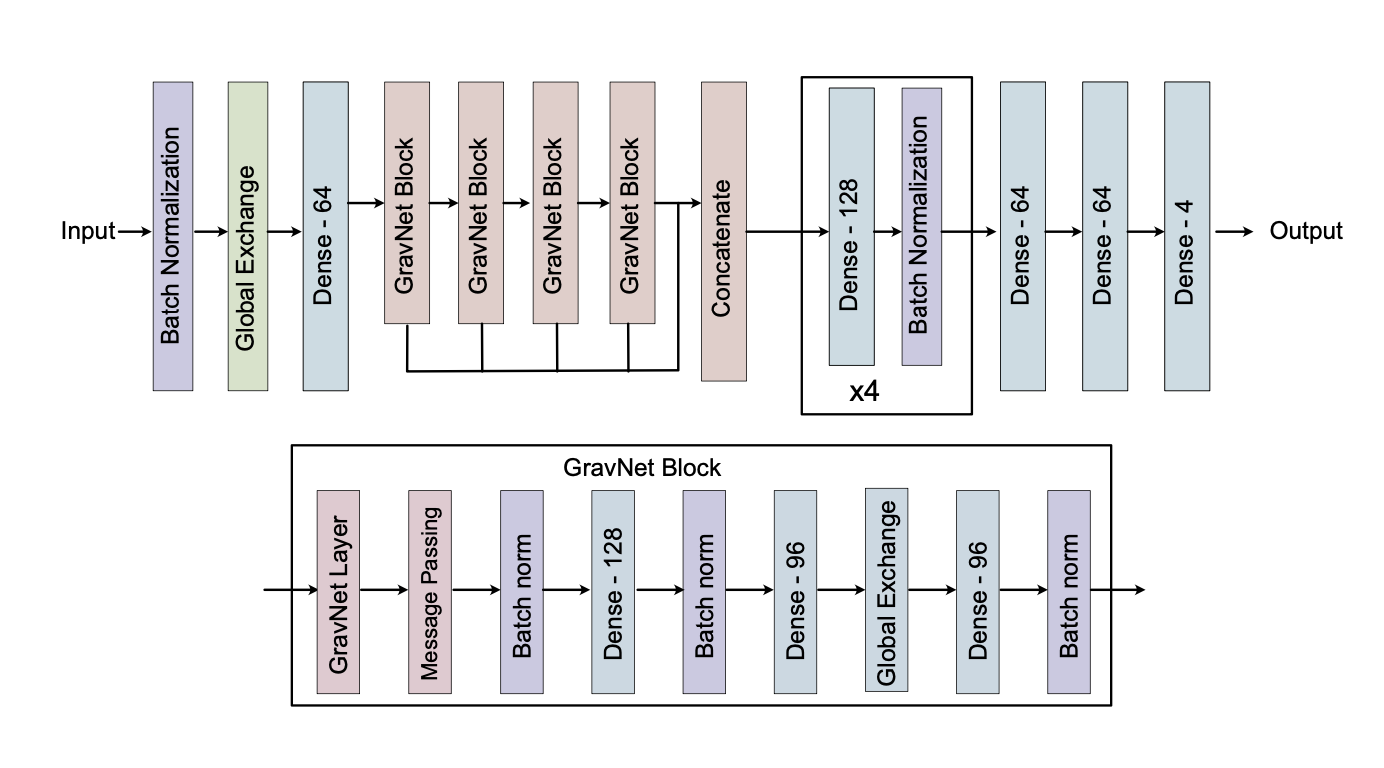
\includegraphics[width=300pt]{./Figure/DLAnalysis/GravArc.png}
		\caption[用いたGravNetアーキテクチャ]{今回用いたGravNetアーキテクチャ。}
		\label{GravArc}
	\end{center}
\end{figure}

入力されたパラメータはまずBatch Normalization, Global Exchange, Dense 層を通過して整形される。Batch Normalizationは過学習を避けるためにBatchごとの出力を規格化する過程である。また、Global Exchange ではバッチごと、特徴量ごとに平均値、最小値、最大値を抽出して入力されたパラメータとconcatenateし、次のレイヤーへと伝達している。これにより、入力されたヒット特徴量の最小や最大、平均といった特徴をより影響しやすくしていると考えられる。Dense層は式(3.1)で表される、線形項と非線形項を組み合わせた全結合層であり、深層ネットワークを構成する基本的な構造の一つである。

その後、GravNet Blockへと移行し、ここではGravNetおよびMessage Passing、 Batch Normalization、 Dense層を含む処理が行われる。GravNet Blockを4回通過した後、Dense 層とBatch Normalizationを同様に4回適用し、最後に3層のDense層を経て出力が得られる。
%このネットワークはGravNetおよびGlobal Exchange、Message Passing以外はヒットの特徴量のみを用いた操作であり、他のNodeとは結合していない。
活性化関数として、GravNet BlockではTanh関数、GravNet Blockの後のDense層ではReLU関数を利用している。また、最適化アルゴリズムとしてAdamWを用いた。これらのネットワーク構造の決定はハイパーパラメータの一種であり、データセットに応じて調整が必要である。


\section{GravNet}

本研究で利用したネットワークについて、その構造と特徴について説明する。

GravNet\cite{GravNet}は、LHCの測定器の一つ CMS (The Compact Muon Solenoid) において、HL-LHC (High Luminosity-LHC)アップグレードで導入される予定のHGCAL (High Granularity CALorimeter) を用いたカロリメータクラスタリングのために開発された深層学習ネットワーク\cite{GravNet_CMS}である。
%欧州原子核研究機構(CERN)の管轄するLHC (Large Hadron Collider)の衝突点付近に置かれる検出器CMS (The Compact Muon Solenoid) 

本研究では入力データとして、カロリメータにおけるヒットの位置およびエネルギー損失を利用する。ヒットの位置は3次元空間上の座標として表現されるので、各ヒットを表す特徴量は今回は4種類存在する。ネットワークに入力されたパラメータはまず全結合層を通過し、その出力をもとにグラフが構成される。全結合層の出力層は、一部はグラフを構成する表現空間の座標に対応し、残りは表現空間における特徴量として利用する。表現空間上の座標を$S$、特徴量を$F_{LR}$とおく。
%表現空間の次元を増やすとより広範な表現能力を獲得できるが、それが過剰になると過学習を起こす危険性が高まる。
ここでは表現空間をSとし、ヒットに対応するグラフのノードのラベルを $(j,k)$とする。ただし、注目するノードをインデックス$k$、そのノードとエッジによって結合したノードをインデックス$j$で表す。さらに、空間S中の2つのノード$(j,k)$間の距離を$d_{jk}$とすると、この距離$d_{jk}$が最も近い$N$個のノードが、エッジによって互いに結合している。

それぞれのノードは周辺のノードから以下の手順に従って特徴量を収集する。

\begin{enumerate}
\item  一つのノードに対して、結合されたノードに与えられた特徴量$f^{i}_{j}$およびノード間の距離$d_{jk}$から、特徴量
\begin{equation}
\tilde{f_{jk}^i} = f^i_j \times V(d_{jk})
\end{equation}
を計算する。ここで、$V(x)$は距離の長さを考慮したポテンシャルを表し、近くのノードほどその影響が大きくなるように設計されている。今回は$V(d_{jk})=\exp(-d_{jk}^2)$を用いた。この計算は一つのノードに対して、結合しているノードの数、すなわち$j$回だけ行われる。

\item 各ノードに対して$\tilde{f_{jk}^i}$を計算した後、それらを concatenate
\footnote{concatenateとは与えられた行列を任意の方向に連結する操作を指す。例として、
\[
A = \begin{pmatrix}
a_1&a_2\\
a_3&a_4\\
\end{pmatrix}
\]
および
\[
B=\begin{pmatrix}
b_1&b_2\\
b_3&b_4\\
\end{pmatrix}
\]
が与えられた時に、
\[
\mathrm{concatenate}(A, B)= 
\begin{pmatrix}
a_1&a_2&b_1&b_2\\
a_3&a_4&b_3&b_4\\
\end{pmatrix}
\]
もしくは
\[
\mathrm{concatenate}(A, B)= 
\begin{pmatrix}
a_1&a_2\\
a_3&a_4\\
b_1&b_2\\
b_3&b_4\\
\end{pmatrix}
\]
となる。
}

することで新たな特徴量$\tilde{f_k^i}$を得る。例えば、$j$個のエッジに対する和や最大値が考えられる。今回は以前行われた研究から得られた結果をもとにして、平均値を利用した。

\item  上記の結果を全てのノードに対して行うことで、$\tilde{f_{k}^i}$を行列要素としてもつ特徴量$\tilde{F_{LR}}$が得られる。この特徴量は入力時に作成された特徴量$F_{\mathrm{IN}}$ベクトルとconcatenateされる。この出力を$F_{\mathrm{OUT}}$と表す。
\end{enumerate}

これらの3つの操作を2回繰り返し、最終的に$F_{\mathrm{IN}}$、$F_{\mathrm{OUT}}$、$F_{\mathrm{OUT}'}$の3つがconcatenateされて出力として得られる。
最終的に計算された出力は各ヒットおよびグラフにより関連づけられたヒットの特徴を表していると考えられる。

\section{Object Condensation}
4.1節で述べた深層学習アーキテクチャを損失関数を用いて学習を行う。今回、アーキテクチャからの出力は$\beta_i$と座標、そしてクラスター特徴量の3種類に分けられている。これらの利用法については以下で述べる。

損失関数として、通常の方法よりも与えられた特徴をさらに効率的に利用するために Object Condensation\cite{GravNet_Object} と呼ばれる手法を用いた。ここで、Condensation pointとは、仮想空間上でそれぞれのクラスターに対して与えられる、それぞれのクラスターに属するヒットが集約する点であり、図\ref{ObjectCondensation}のように現れる。
\begin{figure}[H]
	\begin{center}
		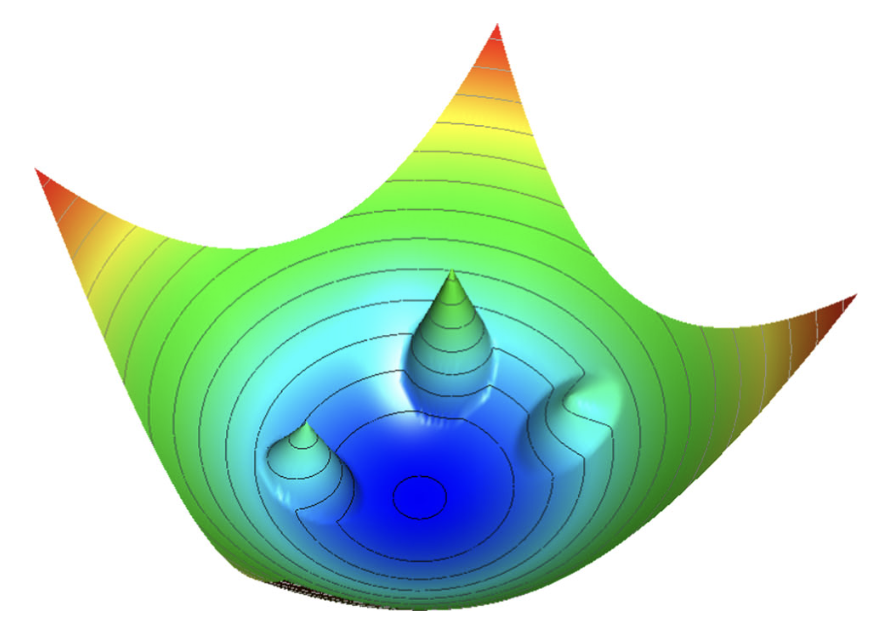
\includegraphics[width=250pt]{./Figure/DLAnalysis/oc.png}
		\caption[ObjectCondensation]{ObjectCondensation\cite{StandardModel}において$L_V$を構成するポテンシャルを模式的に描いた図。突起状に飛び出た部分がCondensation pointと呼ばれる。}
		\label{ObjectCondensation}
	\end{center}
\end{figure}

この手法では、損失関数として次の2つの項を採用し、クラスター識別性能を高めている。
\begin{equation}
L=L_V + L_p
\end{equation}

第一項は全ポテンシャル損失を表す。ネットワークから出力される値は、それぞれのヒットが正しいクラスターに属しているかどうかを示す$\beta_i$となっている。Object condensationはこの値をもとにノードの持つ電荷を定義し、ネットワークのパラメータ更新に用いられる。すなわち、
\begin{equation}
q_i =\arctanh^2\beta_i + q_{min}
\end{equation}
によって電荷$q_i$を定義する。特定のクラスター$k$に属するヒット$i$のもつ$q_i$はポテンシャル$V_{ik}$を有する。
電磁気学のアナロジーから、ヒットが正しいクラスターへ引力によって引き付けられ、誤ったクラスターから斥力によって離れるように学習を行いたい。
そのため、電荷$q_j$とポテンシャル$V_{ik}(x_j,q_j)$を用いて、各ヒットに働く静電気力を以下のように表す。

\begin{equation}
q_j \cdot \Delta V_k(x_j) = q_j \Delta \sum_{i=1}^{N} M_{ik} V_{ik} (x_j ,q_i)
\end{equation}

ここで、行列$M_{ik}$はヒット$i$がクラスター$k$に属している場合は1を、そうでなければ0を表す。この行列は$N\times N$個の要素数を持つので、全てのポテンシャルを計算するのは計算リソースの消費が大きくなるという問題がある。そのため、それぞれのクラスターに含まれるヒットの中から、以下のように最も大きなポテンシャルを持つヒット$i$のポテンシャルによって近似する。

\begin{equation}
V_k(x) \approx V_{\alpha k}(x, q_{\alpha k}),\  with\ q_{\alpha k} = \max q_i M_{ik}  
\end{equation}

すなわち、一つのクラスターのなかでそれぞれのヒットに働くクーロン力はその電荷にのみ依存する。

この表式を用いて、引力および斥力ポテンシャルは以下のように表される。
\begin{equation}
\check{V}(x) = ||x-x_{\alpha} ||^2 q_{\alpha k}
\end{equation}
\begin{equation}
\hat{V}_{k}(x) = \max(0,1-||x-x_\alpha ||)q_{\alpha k}
\end{equation}

前者のポテンシャルにより、それぞれのヒットは各クラスターに割り当てられた Condensation point$||x-x_{\alpha}||=0$へと集められる。一方、誤ったクラスターに近づいている場合は後者のポテンシャルによってそのクラスターから引き離される。斥力ポテンシャルに関して、ポテンシャルが大局的鞍点とは異なる局所的な平衡点へとどまりパラメータ更新が進みにくくなるのを防ぐためにポテンシャルと0を比較した時の最大値を採用した。

上記の2つの項を合わせて、損失関数のポテンシャル項は以下のように表される。
\begin{equation}
L_V = \frac{1}{N}\sum_{j=1}^{N} q_j \sum_{k=1}^K \left(M_{jk} \check{V}_k(x_j) + (1 - M_{jk})\hat{V}_k(x_j)\right)
\end{equation}

この損失関数は$||x-x_{\alpha}|| = 0$に鞍点をもち、同じクラスターに属するヒットはその中で最も電荷の高いヒットへと引っ張られる。一方、そのクラスターに属さないヒットは離れた位置へと押しやられる。

式(4.2)の第2項はベータ損失と呼ばれ、先ほど定義した各クラスターを代表するヒットの持つ$\beta$の値を最大化するために用いられており、以下で定義される。
\begin{equation}
L_\beta = \frac{1}{K}\sum_k (1-\beta_{\alpha k}) +s_B \frac{1}{N_B}\sum_i^N n_i \beta_i
\end{equation}
ここで、$s_B$はハイパーパラメータであり、データセットごとに異なる値を取る必要がある。この項の存在によって、それぞれのヒットのCondensation pointの影響が強調され、バックグラウンドやノイズの影響が低減される。$s_B$はバックグラウンドを低減させる強さを示し、全てのクラスターが正しくラベル付けされていれば大きく設定する。


\section{ILCの検出器シミュレーションデータを用いたカロリメトリー}
この章では、シミュレーションフレームワークの一つであるWHIZARDおよびILD検出器シミュレーション(iLCSoft v02-02)を用いて生成された2光子イベントのGravNetによるクラスタリングについて述べる。4.2.1節で入力データについて述べた後、4.2.2節でネットワークの評価を行う。

%%%%%%%%%%%%%%%%%%%%%%%%%%%%%%%%%%%%%%%%%%%%%%%%%%%%%%%%%%%%%%%%%%%%%%%%%%%%%%%%%%%%
\begin{comment}
\subsection{入力データ}
今回使用したデータは重心エネルギー$\SI{500}{GeV}$におけるZ粒子の崩壊を通じたハドロニック事象である。 シミュレーションにおいて、反応により生じた光子や中性ハドロンなどの粒子がILDのEcalおよびHcalへ入射し、電磁シャワーやハドロンシャワーを引き起こす。今回は1600事象を含むデータを用意した。

検出器シミュレーションにより出力されるのは各ヒットの位置、エネルギー損失やその生成元となるMC粒子の情報を持ったLCIOファイルである。LCIOファイルはPythonによって読み込みが可能であるが、深層学習を適用するためにはデータの剪定と事前処理が必要である。データを読み込む際に毎回この処理を行うと時間がかかりすぎるので、このファイルをPythonコードにより変換し、各事象ごとにnpzファイルを作成した。npzファイルにはヒットの情報として位置($x$,$y$,$z$)および各エネルギー損失が含まれる。ヒットの時間情報は今回は使用しなかった。正解ラベルとして、各ヒットが生成されたMC粒子のIDをもとにした番号を割り当てた。番号はMC粒子の種類に関わらず、0から昇順に生成された。

図\ref{Input}、\ref{EnergyDep}にある一つのイベントに含まれる各ヒットの位置およびエネルギー損失の情報を示す。ヒット位置のプロットに関して、原点がビーム衝突位置である。

\begin{figure}[H]
	\begin{subfigure}{.5\textwidth}
		\begin{center}
 		 	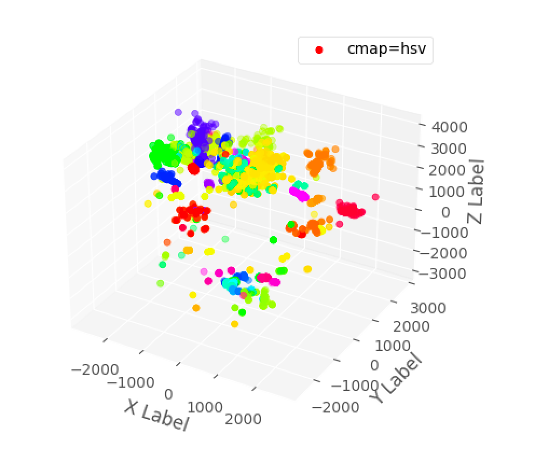
\includegraphics[width=200pt]{./Figure/DLAnalysis/Input.png}%.5\linewidth]{./Figure/DLAnalysis/Input2.png}
  			\caption{}
  			\label{fig:sfig1}
 		\end{center}
	\end{subfigure}
	\begin{subfigure}{.5\textwidth}
		\begin{center}
			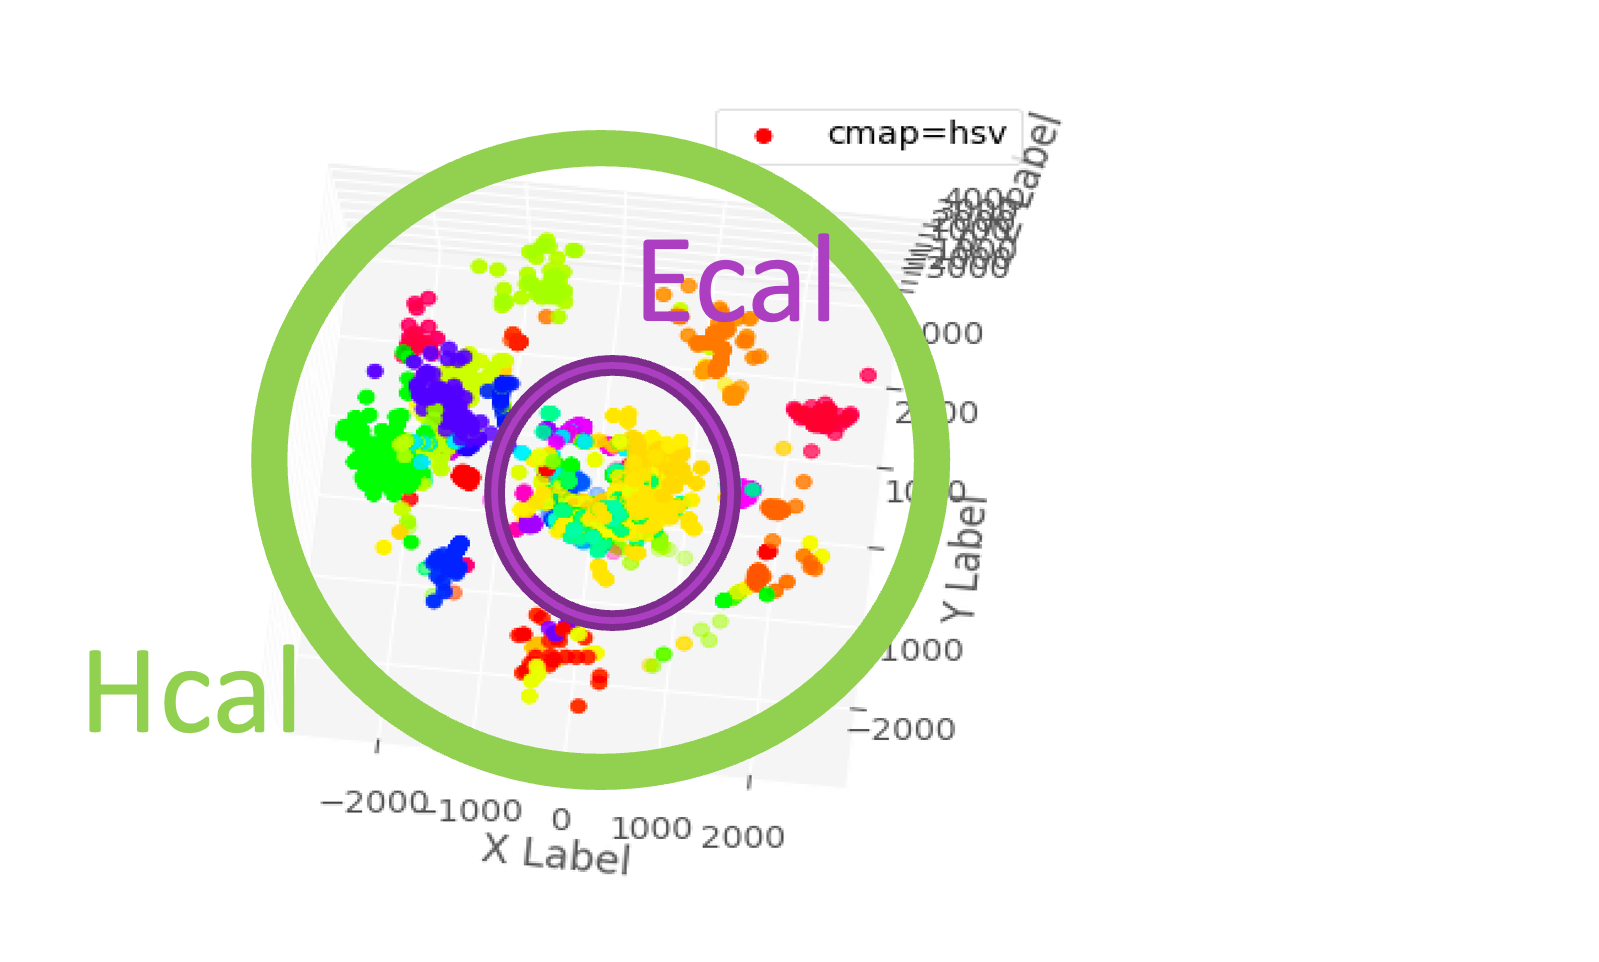
\includegraphics[width=250pt]{./Figure/DLAnalysis/Input2.png}%.5\linewidth]{./Figure/DLAnalysis/Input2.png}
			\caption{}
			\label{fig:sfig2}
		\end{center}
	\end{subfigure}
	\caption[入力データのヒット位置]{入力データのヒット位置の一例。(b)は(a)を上方向から見た図。EcalとHcalがそれぞれ含まれているのがわかる。}
	\label{Input}
\end{figure}

\begin{figure}[H]
	\begin{center}
		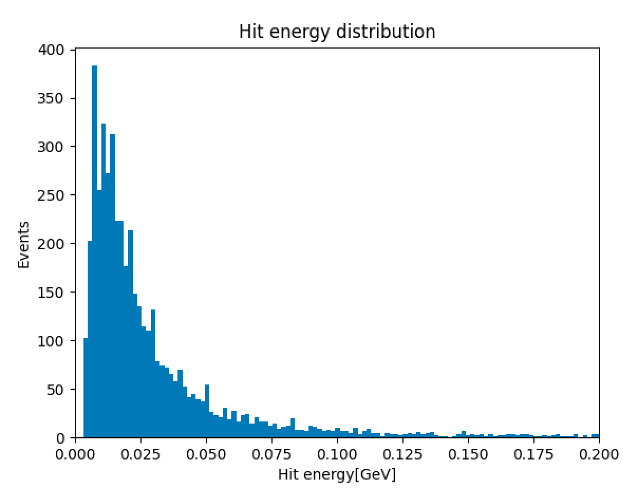
\includegraphics[width=250pt]{./Figure/DLAnalysis/Energydep.png}
		\caption[入力データのエネルギー損失]{シミュレーションデータのエネルギー損失の一例。}
		\label{EnergyDep}
	\end{center}
\end{figure}


入力データの事前処理として、パラメータの規格化をおこない、データ範囲が$[-1,1]$となるように調整した。ヒット位置はカロリメータの位置から$[-2000,2000]$の範囲に制限されているので、2000で除算をおこなった。一方、エネルギー損失については tanh関数で圧縮した。
以下にこれらのパラメータ整形をまとめる。

\begin{enumerate}
\item ヒットの位置
\[
(x',y',z') = \left(\frac{x}{2000},\frac{y}{2000},\frac{z}{2000}\right) 
\]
\item ヒットのエネルギー損失
\[
E' = \tanh(E)
\]
\end{enumerate}


\subsection{ネットワークの評価}
ネットワークの評価として、エポックに対する損失関数の変化と表現空間における1つのイベントのヒット分布を確認した。

訓練データおよび評価データの各エポックごとの損失関数は図\ref{Loss_ILD}のように推移した。

\begin{figure}[H]
	\begin{center}
		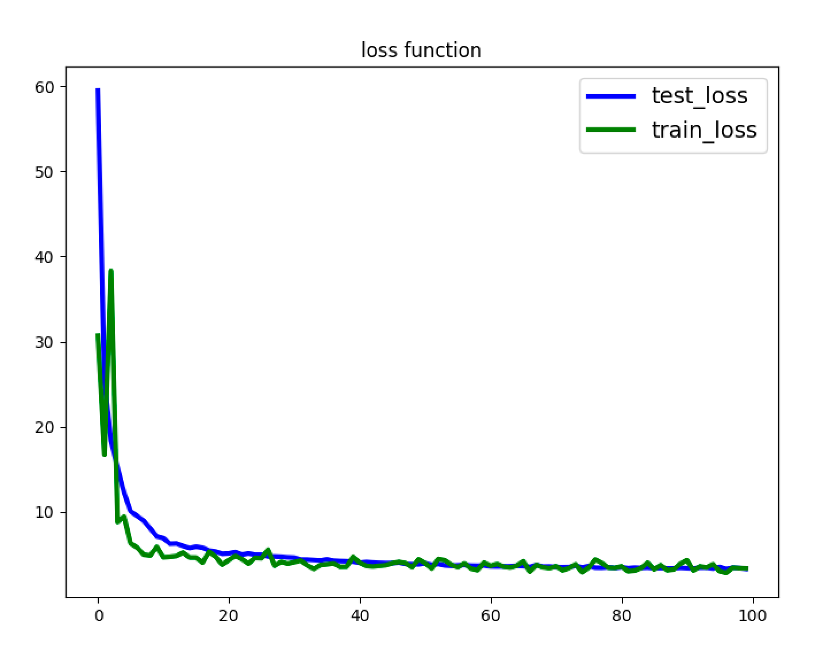
\includegraphics[width=250pt]{./Figure/DLAnalysis/Loss_ILD.png}
		\caption[損失関数の推移]{損失関数の推移。}
		\label{Loss_ILD}
	\end{center}
\end{figure}

どちらのデータも均等に損失関数が減少しており、適切に学習が行えていることがわかる。

また、ネットワークの評価として、Object Condensationから出力されたヒットの表現空間において、各クラスターが異なる位置に分類されているかどうかを確認した。学習前のプロットと30エポック学習後の表現空間が図\ref{representation}に示されている。

\begin{figure}[H]
	\begin{subfigure}{.5\textwidth}
		\begin{center}
 		 	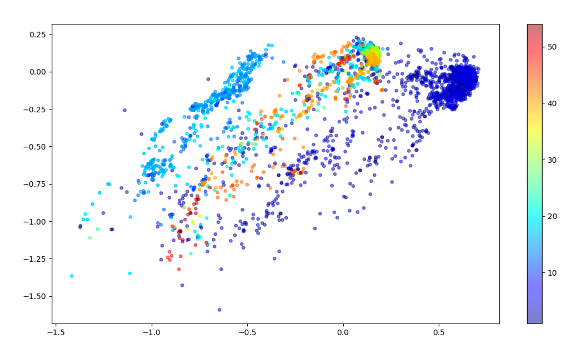
\includegraphics[width=200pt]{./Figure/DLAnalysis/Repre_before.png}%.5\linewidth]{./Figure/DLAnalysis/Input2.png}
  			\caption{}
  			\label{fig:sfig1}
 		\end{center}
	\end{subfigure}
	\begin{subfigure}{.5\textwidth}
		\begin{center}
			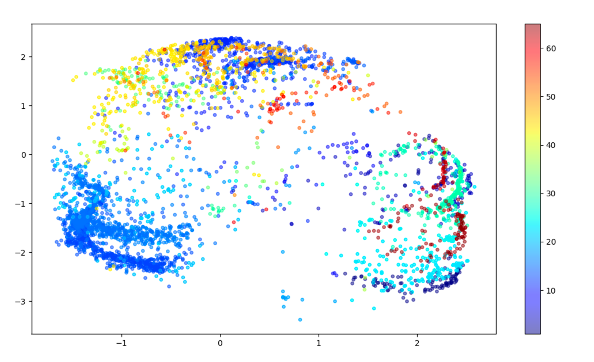
\includegraphics[width=200pt]{./Figure/DLAnalysis/Repre_30.png}%.5\linewidth]{./Figure/DLAnalysis/Input2.png}
			\caption{}
			\label{fig:sfig2}
		\end{center}
	\end{subfigure}
	\caption[学習前と30エポック学習後の表現空間の比較]{学習前と30エポック学習後の表現空間の比較。}
	\label{representation}
\end{figure}


それぞれの点がヒットを示しており、色がクラスター分けを示す。学習前のプロットにおいても学習後のプロットにおいても3つの分布に分かれていることが分かるが、学習後の方が表現空間におけるそれぞれのクラスター間の距離が大きくなっている。これは異なるクラスターを識別するためにそれぞれのクラスターに属するヒットの特徴量がネットワークにより学習されていることを示している。しかし表現空間における3つの分布の中に含まれるそれぞれのクラスターは十分に分けられていない。


\section{2光子事象を用いたカロリメトリー}
%%%%%%%%%%%%%%%%%%%%%%%%%%%%%%%%%%%%%%%%%%%%%%%%%%%%%%%%%%%%%%%%%%%%%%%%%%%%%%%%%%%%%%%%%%%%%
\end{comment}
\subsection{入力データ}
入力データとして、近接する2光子イベントの検出器シミュレーションデータを作成した。ビーム衝突点から特定の角度で2本の光子を入射させ、極角を$\SI{85}{rad}$に固定し方位角$\phi$をランダムに取ることで訓練用及び評価用のデータを作成した。角度は$\SI{1/10}{ rad}$の識別のより困難なケースから$\SI{5/10}{ rad}$のより容易なケースまで、$\SI{0.1}{rad}$ずつ、5つのファイルをそれぞれ20000イベント用意した。光子の運動量は$\SI{5}{GeV}$、検出器シミュレーションにより出力されるのは各ヒットの位置、エネルギー損失やその生成元となるモンテカルロシミュレーション(Monte Carlo simulation, MC)粒子の情報を持ったLCIOファイルである。LCIOファイルはPythonによって読み込みが可能であるが、深層学習を適用するためにはデータの選定と事前処理が必要である。データを読み込む際に毎回この処理を行うと時間がかかりすぎるので、このファイルをPythonコードにより変換し、各イベントごとに深層学習に適したフォーマットであるnpzファイルを作成した。npzファイルにはヒットの情報として位置($x$,$y$,$z$)および各エネルギー損失が含まれる。ヒットの時間情報は今回は使用しなかった。正解ラベルとして、各ヒットが生成されたMC粒子のIDをもとにした番号を割り当てた。番号はMC粒子の種類に関わらず、0から昇順に生成された。

図\ref{DoublePG}にこのデータの概形を示す。

\begin{figure}[H]
	\begin{subfigure}{.5\textwidth}
		\begin{center}
 		 	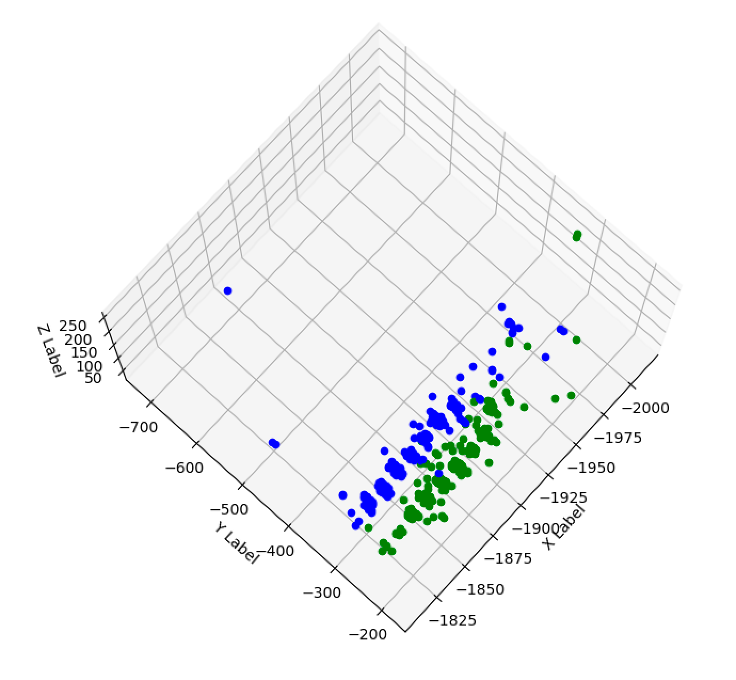
\includegraphics[width=200pt]{./Figure/DLAnalysis/Double1.png}%.5\linewidth]{./Figure/DLAnalysis/Input2.png}
  			\caption{}
  			\label{fig:sfig1}
 		\end{center}
	\end{subfigure}
	\begin{subfigure}{.5\textwidth}
		\begin{center}
			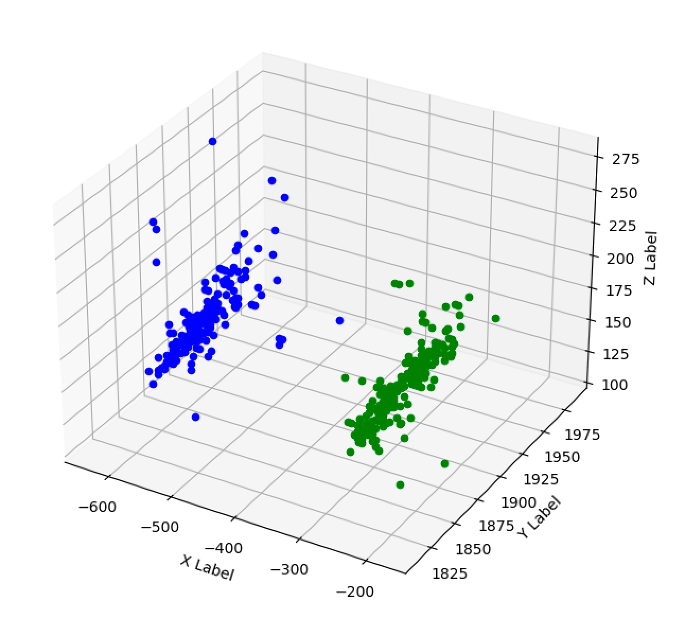
\includegraphics[width=200pt]{./Figure/DLAnalysis/Double5.png}%.5\linewidth]{./Figure/DLAnalysis/Input2.png}
			\caption{}
			\label{fig:sfig2}
		\end{center}
	\end{subfigure}
	\caption[DoubleParticleGunによる$\SI{0.5}{rad}$および$\SI{0.1}{rad}$の場合の入力データのヒット位置]{$\SI{0.5}{rad}$および$\SI{0.1}{rad}$の場合の入力データのヒット位置。}
	\label{DoublePG}
\end{figure}

入力データの事前処理として、パラメータの規格化をおこない、データ範囲が$[-1,1]$となるように調整した。ヒット位置はカロリメータの位置から$[-2000,2000]$の範囲に制限されているので、2000で除算をおこなった。一方、エネルギー損失については tanh関数で圧縮した。
以下にこれらのパラメータ整形をまとめる。

\begin{enumerate}
\item ヒットの位置
\[
(x',y',z') = \left(\frac{x}{2000},\frac{y}{2000},\frac{z}{2000}\right) 
\]
\item ヒットのエネルギー損失
\[
E' = \tanh(E)
\]
\end{enumerate}
訓練用データとして、全データの80\%にあたる80000イベントを用い、評価用データとして残りの20000イベントを使用した。学習は各角度で行い、同じ角度で推論を行った。

\subsection{ネットワークの評価}
ネットワークの評価として、Object Condensationから出力された$\beta_i$をもとに各々のヒットをクラスター分けし、それらを3Dプロット上で正解ラベルと比較した。

図\ref{DoublePG_5_res}は2光子の角度が$\SI{0.5}{rad}$の場合のプロットである。図(a)は良くクラスタリングできている例を示している。一方、図(b)は一つのヒットが異なって識別されているものを示した。図(b)から、二つのクラスターの境界付近において識別がやや困難になっている可能性がある。

\begin{figure}[H]
	\begin{subfigure}{.5\textwidth}
		\begin{center}
 		 	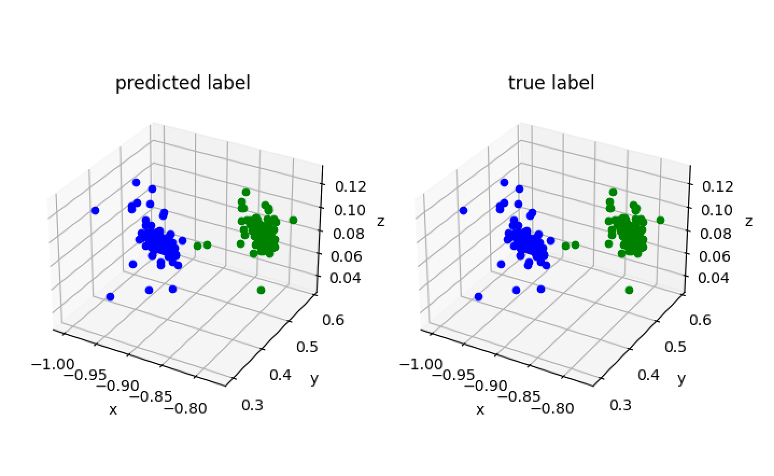
\includegraphics[width=200pt]{./Figure/DLAnalysis/Double5_1.png}%.5\linewidth]{./Figure/DLAnalysis/Input2.png}
  			\caption{}
  			\label{DPG_res_a}
 		\end{center}
	\end{subfigure}
	\begin{subfigure}{.5\textwidth}
		\begin{center}
			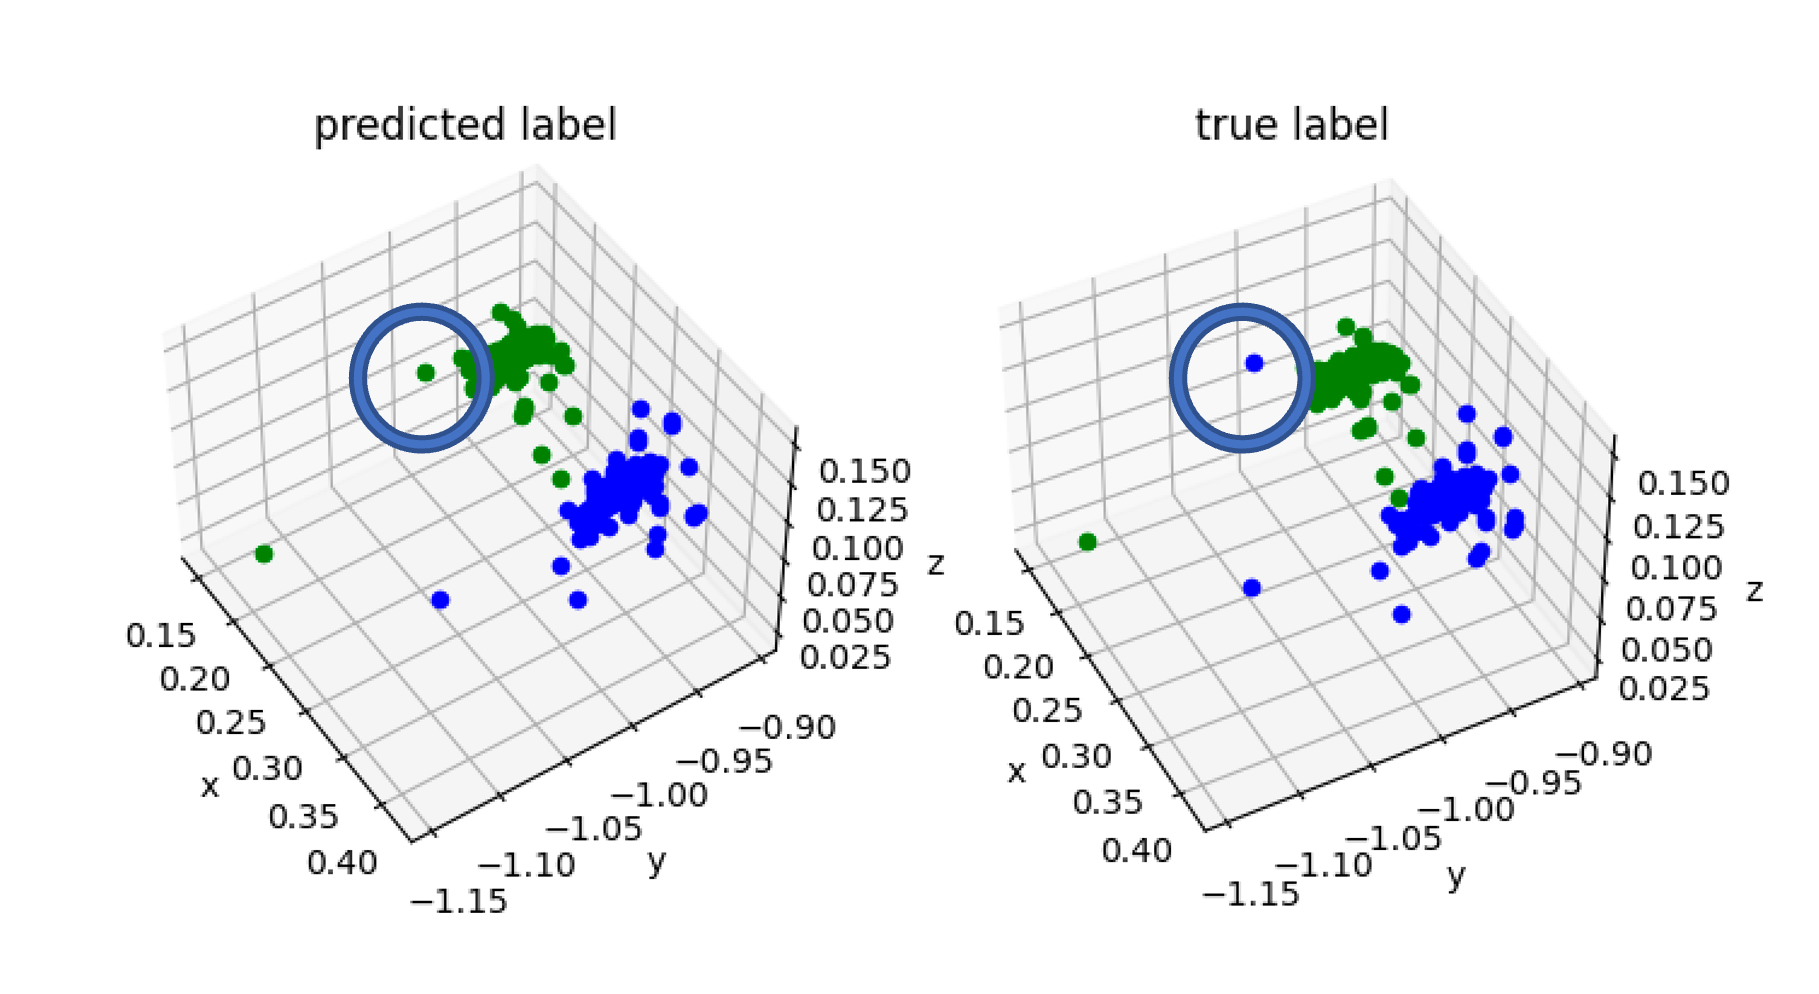
\includegraphics[width=200pt]{./Figure/DLAnalysis/Double5_2.png}%.5\linewidth]{./Figure/DLAnalysis/Input2.png}
			\caption{}
			\label{DPG_res_b}
		\end{center}
	\end{subfigure}
	\caption[$\SI{0.5}{rad}$の場合の比較]{$\SI{0.5}{rad}$の場合のネットワークにより予測されたラベルと正解ラベルの比較。(a)は全てのヒットが正しく識別できている場合。(b)は一つのヒットが誤って識別されている場合。}
	\label{DoublePG_5_res}
\end{figure}

図\ref{DoublePG_1_res}は2光子の角度が$\SI{0.1}{rad}$の場合の場合のプロットである。先ほどとは異なり、多くのイベントは図のように3つにクラスタリングされており、先ほどのケースよりも識別が難しいことを確認した。
\begin{figure}[H]
	\begin{subfigure}{.5\textwidth}
		\begin{center}
 		 	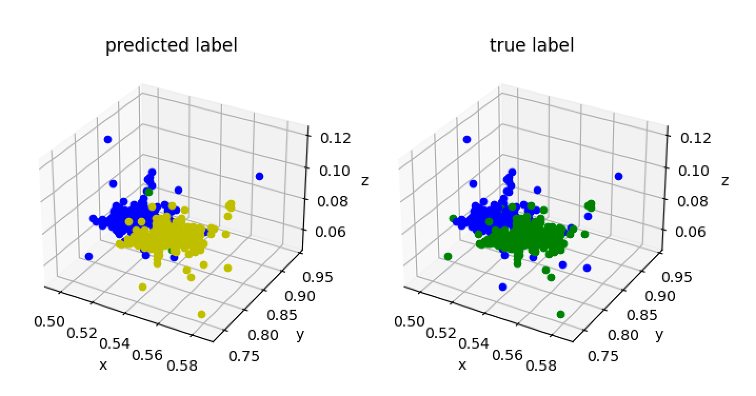
\includegraphics[width=200pt]{./Figure/DLAnalysis/Double1_2.png}%.5\linewidth]{./Figure/DLAnalysis/Input2.png}
  			\caption{}
  			\label{DPG_res_a}
 		\end{center}
	\end{subfigure}
	\begin{subfigure}{.5\textwidth}
		\begin{center}
			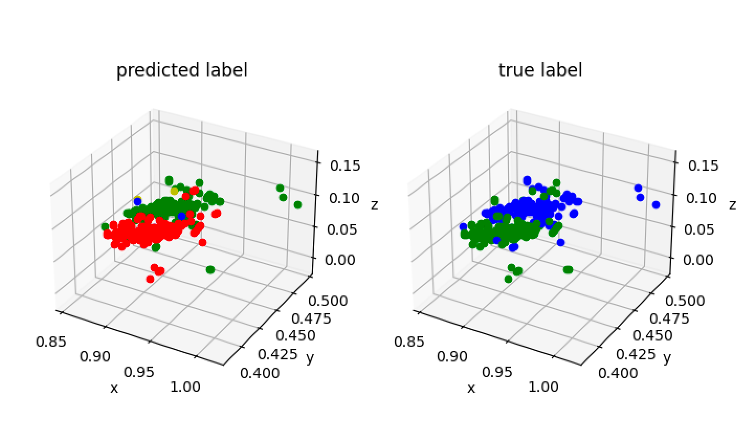
\includegraphics[width=200pt]{./Figure/DLAnalysis/Double1_1.png}%.5\linewidth]{./Figure/DLAnalysis/Input2.png}
			\caption{}
			\label{DPG_res_b}
		\end{center}
	\end{subfigure}
	\caption[$\SI{0.5}{rad}$の場合の場合の比較]{$\SI{0.5}{rad}$の場合のネットワークにより予測されたラベルと正解ラベルの比較。(a)、(b)ともにいくつかのヒットが誤って識別されている。}
	\label{DoublePG_1_res}
\end{figure}

これらのイベントの中には光子が変換して他のMC粒子が生成されているものもあったが、それらについては正解ラベルの数が3以上のものを基準として除外している。

次に、定量的にクラスタリングの精度を以下の式で定義し、比較を行った。
\begin{equation}
\textrm{accuracy} = \frac{\textrm{predicted\ hit\ with\ correct\ label}}{\textrm{true\ label}}
\end{equation}

5つのシミュレーションデータに対して、イベントに含まれるクラスターごとに上記の値を計算し、全イベントにわたってプロットしたものを図\ref{result_DoublePG}に示す。

\begin{figure}[H]
	\begin{subfigure}{.5\textwidth}
		\begin{center}
 		 	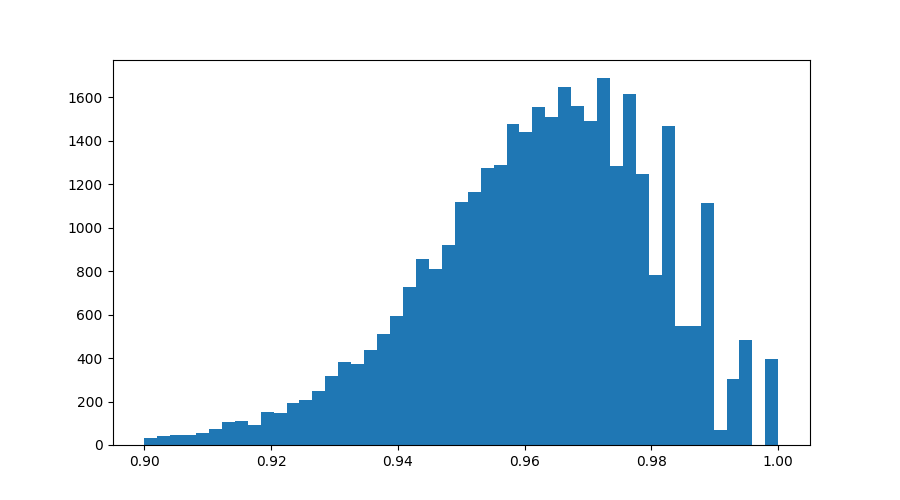
\includegraphics[width=200pt]{./Figure/DLAnalysis/rate_pred_1.png}%.5\linewidth]{./Figure/DLAnalysis/Input2.png}
  			\caption{$\SI{0.1}{rad}$}
  			\label{fig:sfig1}
 		\end{center}
	\end{subfigure}
	\begin{subfigure}{.5\textwidth}
		\begin{center}
			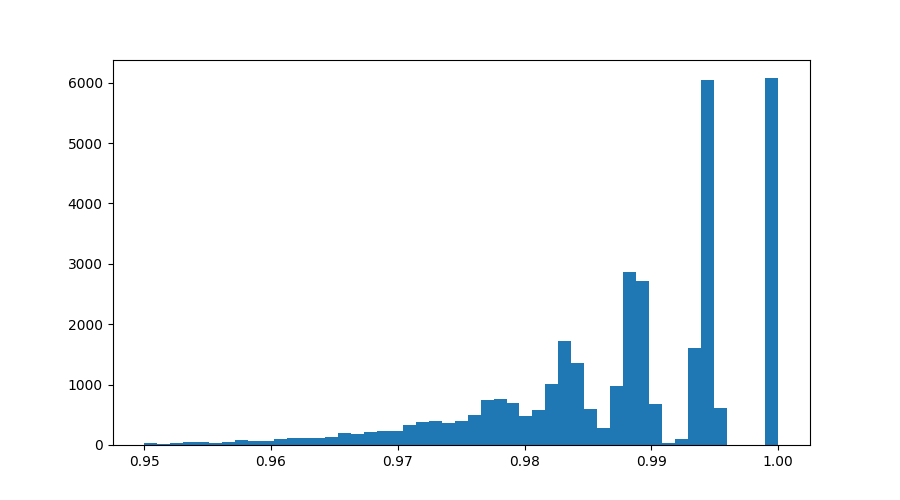
\includegraphics[width=200pt]{./Figure/DLAnalysis/rate_pred_2.png}%.5\linewidth]{./Figure/DLAnalysis/Input2.png}
			\caption{$\SI{0.2}{rad}$}
			\label{fig:sfig2}
		\end{center}
	\end{subfigure}
		\begin{subfigure}{.5\textwidth}
		\begin{center}
			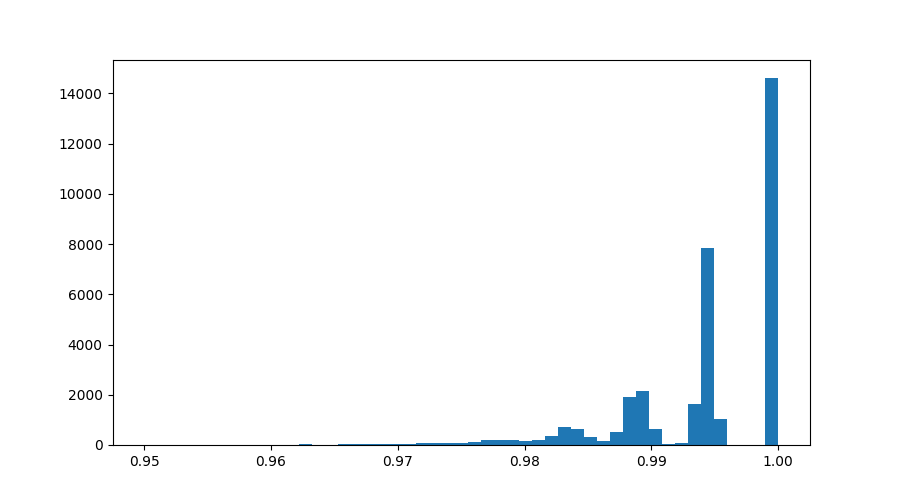
\includegraphics[width=200pt]{./Figure/DLAnalysis/rate_pred_3.png}%.5\linewidth]{./Figure/DLAnalysis/Input2.png}
			\caption{$\SI{0.3}{rad}$}
			\label{fig:sfig2}
		\end{center}
	\end{subfigure}
		\begin{subfigure}{.5\textwidth}
		\begin{center}
			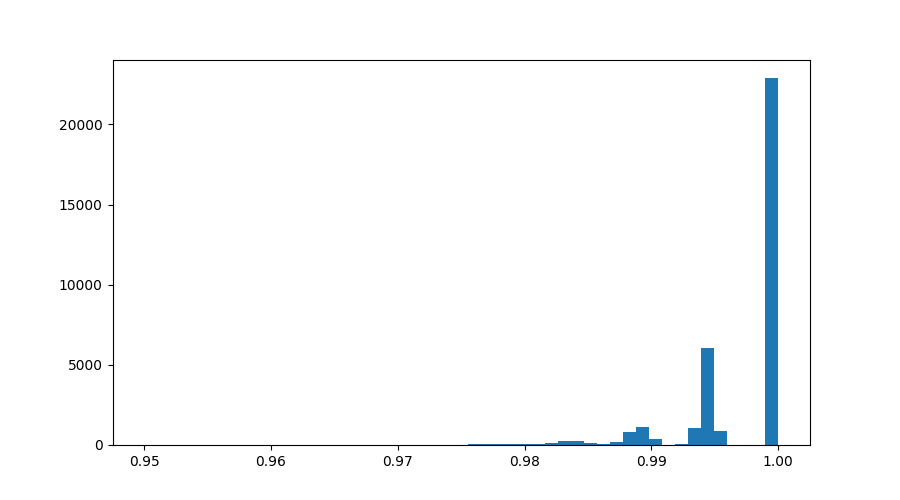
\includegraphics[width=200pt]{./Figure/DLAnalysis/rate_pred_4.png}%.5\linewidth]{./Figure/DLAnalysis/Input2.png}
			\caption{$\SI{0.4}{rad}$}
			\label{fig:sfig2}
		\end{center}
	\end{subfigure}
	\begin{subfigure}{.5\textwidth}
		\begin{center}
			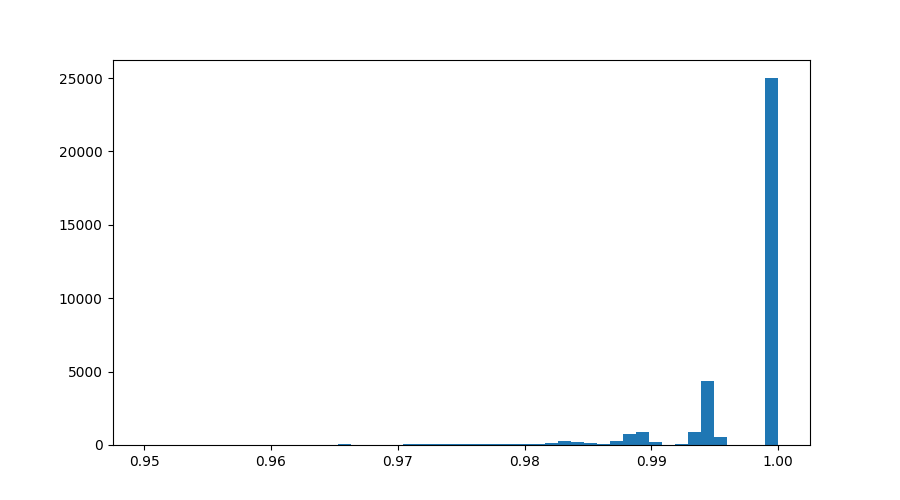
\includegraphics[width=200pt]{./Figure/DLAnalysis/rate_pred_5.png}%.5\linewidth]{./Figure/DLAnalysis/Input2.png}
			\caption{$\SI{0.5}{rad}$}
			\label{fig:sfig2}
		\end{center}
	\end{subfigure}

	\caption[2光子事象による$\SI{0.1}{rad}$から$\SI{0.5}{rad}$までのシミュレーションデータの各クラスターごとの正しく識別できたヒット数]{2光子事象による$\SI{0.1}{rad}$から$\SI{0.5}{rad}$までのシミュレーションデータの各クラスターごとの正しく識別できたヒット数。横軸はaccuracy、縦軸はクラスター数を表す。}
	\label{result_DoublePG}
\end{figure}

%%%%%%%%%%%%%%%%%%%%%%%%%%%%%%%%%%%%%%%%%%%%%%%%%%%%%%%%%%%%%%%%%%%%%%
\begin{comment}
\begin{figure}[H]
	\begin{center}
		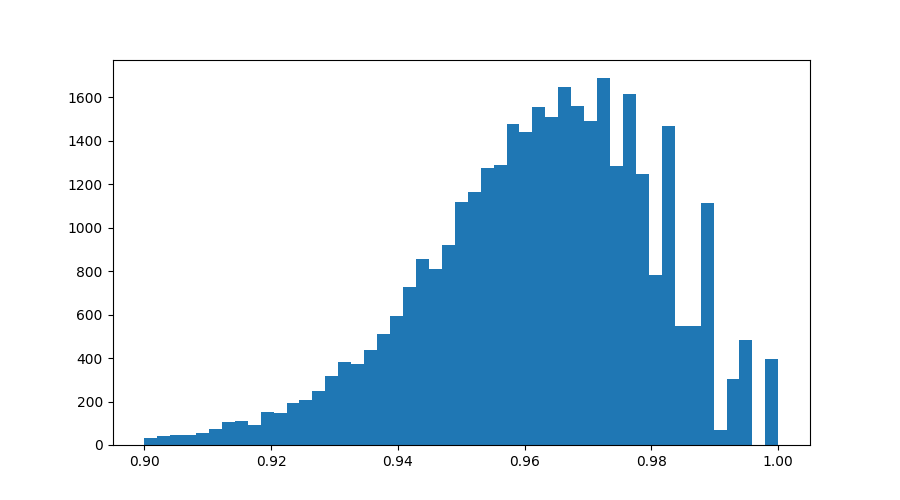
\includegraphics[width=250pt]{./Figure/DLAnalysis/rate_pred_1.png}
		\caption[角度$\SI{0.1}{rad}$のシミュレーションデータの各クラスターごとの正しく識別できたヒット数]{角度$\SI{0.1}{rad}$のシミュレーションデータの各クラスターごとの正しく識別できたヒット数。横軸は縦軸がクラスターの数}
		\label{result_DoublePG1}
	\end{center}
\end{figure}

\begin{figure}[H]
	\begin{center}
		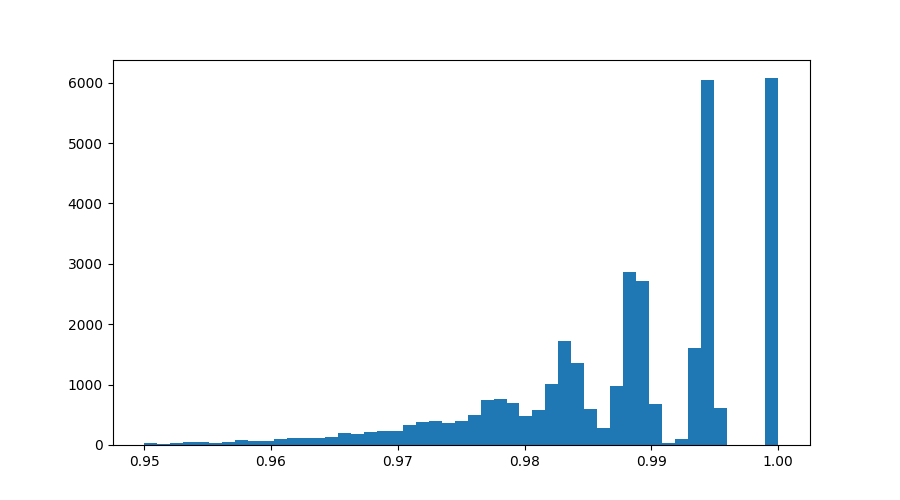
\includegraphics[width=250pt]{./Figure/DLAnalysis/rate_pred_2.png}
		\caption[角度$\SI{0.2}{rad}$のシミュレーションデータの各クラスターごとの正しく識別できたヒット数]{角度$\SI{0.2}{rad}$のシミュレーションデータの各クラスターごとの正しく識別できたヒット数。}
		\label{result_DoublePG2}
	\end{center}
\end{figure}

\begin{figure}[H]
	\begin{center}
		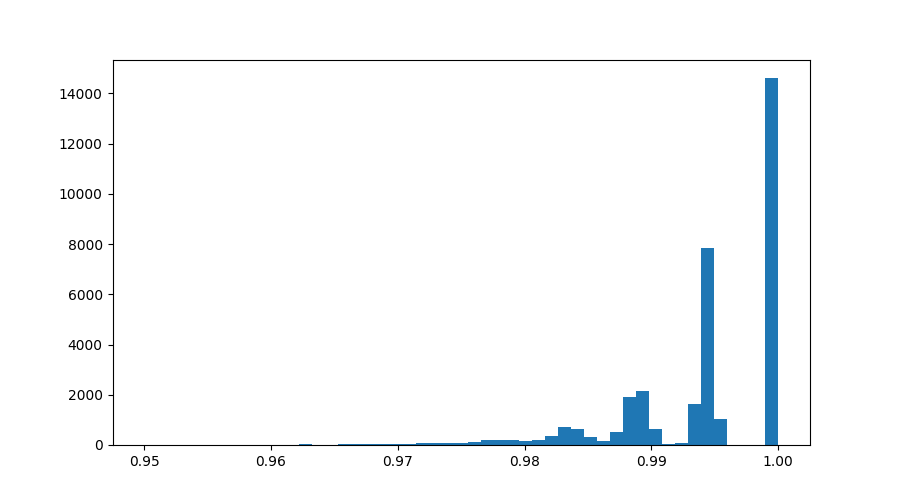
\includegraphics[width=250pt]{./Figure/DLAnalysis/rate_pred_3.png}
		\caption[角度$\SI{0.3}{rad}$のシミュレーションデータの各クラスターごとの正しく識別できたヒット数]{角度$\SI{0.3}{rad}$のシミュレーションデータの各クラスターごとの正しく識別できたヒット数。}
		\label{result_DoublePG3}
	\end{center}
\end{figure}

\begin{figure}[H]
	\begin{center}
		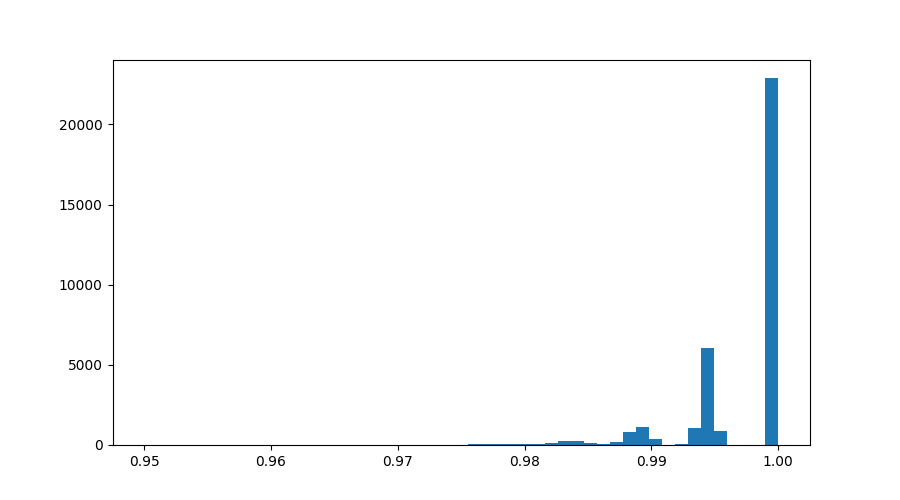
\includegraphics[width=250pt]{./Figure/DLAnalysis/rate_pred_4.png}
		\caption[角度$\SI{0.4}{rad}$のシミュレーションデータの各クラスターごとの正しく識別できたヒット数]{角度$\SI{0.4}{rad}$のシミュレーションデータの各クラスターごとの正しく識別できたヒット数。}
		\label{result_DoublePG4}
	\end{center}
\end{figure}

\begin{figure}[H]
	\begin{center}
		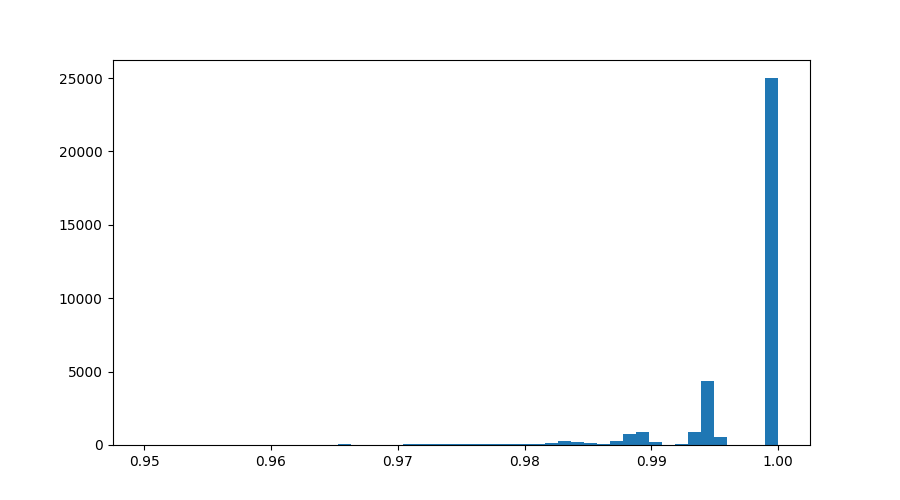
\includegraphics[width=250pt]{./Figure/DLAnalysis/rate_pred_5.png}
		\caption[角度$\SI{0.5}{rad}$のシミュレーションデータの各クラスターごとの正しく識別できたヒット数]{角度$\SI{0.5}{rad}$のシミュレーションデータの各クラスターごとの正しく識別できたヒット数。}
		\label{result_DoublePG5}
	\end{center}
\end{figure}
\end{comment}
%%%%%%%%%%%%%%%%%%%%%%%%%%%%%%%%%%%%%%%%%%%%%%%%%%%%%%%%%%%%%%%%%%%%%%%%%%%%%%%%%


各イベントごとに測定された、各クラスターの精度の平均値を表\ref{acc_Grav}にまとめる。

\begin{table}[h]
	\begin{center}
		\begin{tabular}{|c|c|c|c|c|c|}
		\hline
		角度$[\SI{}{rad}]$&0.1&0.2&0.3&0.4&0.5\\\hline\hline
		accuracy[\%]&96.08&98.64&99.30&99.68&99.56\\\hline
		\end{tabular}
	\end{center}
	\caption[角度ごとの各クラスターの精度の平均値]{角度ごとの各クラスターの精度の平均値。}
\label{acc_Grav}
\end{table}

$\SI{0.5}{rad}$のデータは99.56\%の精度を達成しているが、角度が小さくなるにつれ精度は悪化し、$\SI{0.1}{rad}$の時点では96.08\%まで減少している。これはシャワーの重なりが大きくなったことで識別が難しくなっているために生じていると考えられる。また、各ヒストグラムについて分布に離散的な飛びが生じているのが確認できる。これはそれぞれの山ごとに誤ってラベルが付けられたヒットの数が1個、2個、$\cdots$と対応していることが考えられる。さらに、本来識別が容易な$\SI{0.5}{rad}$のクラスターよりも$\SI{0.4}{rad}$の方が精度が高くなっている。それぞれのヒストグラムを見ると、(d)に含まれるピークは(e)に含まれるピークよりも全体的に少なくなっているように見える。このことから、原因としてはデータの揺らぎによる影響だけでなく、$\SI{0.4}{rad}$のイベントの中に光子が変換されて生じた正解ラベルクラスターの数が3以上のものが多く含まれているために、全体のイベント数に偏りが生じているためではないかと考えた。これを確かめるためには実際にカットされなかったイベント数を数える必要がある。

さらに、今回は2つの光子のみの単純なデータであったが、実際のILDへ適用するにあたり、さらに複雑なシミュレーションデータを用意し、性能評価および最適化をする必要があると考える。


%およそ70\%のクラスターに含まれるヒットが正しくラベルを識別できていることがわかる。
%残りの30\%のクラスターについて、なぜラベルを識別できていないか確認するために一つのイベントについて図のように3Dプロットで確認した。

%本手法は後述するEBES実験における2光子検出に対しても有効であり、本研究はその応用に向けた初期研究である。
